\documentclass{article}
\usepackage{amsmath}
\usepackage{amsfonts}
\usepackage{amssymb}
\usepackage{listings}
\usepackage{xcolor}
\usepackage{parskip}
\usepackage{graphicx}
\usepackage{float}

\definecolor{codegreen}{rgb}{0,0.6,0}
\definecolor{codegray}{rgb}{0.5,0.5,0.5}
\definecolor{codepurple}{rgb}{0.58,0,0.82}
\definecolor{backcolour}{rgb}{0.95,0.95,0.92}

\lstdefinestyle{mystyle}{
    backgroundcolor=\color{backcolour},   
    commentstyle=\color{codegreen},
    keywordstyle=\color{magenta},
    numberstyle=\tiny\color{codegray},
    stringstyle=\color{codepurple},
    basicstyle=\ttfamily\footnotesize,
    breakatwhitespace=false,         
    breaklines=true,                 
    captionpos=b,                    
    keepspaces=true,                 
    numbers=left,                    
    numbersep=5pt,                  
    showspaces=false,                
    showstringspaces=false,
    showtabs=false,                  
    tabsize=2
}
\lstset{style=mystyle}
\usepackage[utf8]{inputenc}

\title{%
  Project 1 - Flow in a driven cavity and non-conforming mesh coupling \\
  \bigskip
  \large Numerics for Fluids, Structures and Electromagnetics}

\author{Mathieu Grondin, Moritz Waldleben}
\date{January 2022}

\begin{document}

\maketitle

\section*{Introduction}
We consider the following Stokes problem on the domain $\Omega \subset
\mathbf{R}^2$ for the velocity $\mathbf{u} : \Omega \rightarrow \mathbb{R}^2$
and the pressure $p:\Omega \rightarrow \mathbb{R}$ :
\begin{align} \label{problem} 
    -\Delta \mathbf{u} + \nabla p &= \mathbf{f}  \quad\textrm{in } \Omega\nonumber\\ 
    \textrm{div} \mathbf{u} &= 0 \quad \textrm{in } \Omega \\
    \mathbf{u} &= \mathbf{g} \quad \textrm{on } \partial \Omega  \nonumber
\end{align}
where $\mathbf{f} : \Omega \rightarrow \mathbb{R}^2$ and $\mathbf{g} :
\partial\Omega\rightarrow\mathbb{R}^2$ are two given function. In particular
assume that $\mathbf{f} \in [H^{-1}(\Omega)]^2=\mathbf{H}^{-1}(\Omega)$ and
$\mathbf{g} \in [H^{1/2}(\partial\Omega)]^2=\mathbf{H}^{1/2}(\partial\Omega)$.

This problem corresponds to solving a flow of an incompressible fluid where
viscous forces dominate inertial forces (i.e. low Reynolds number). The
equations are essentially stationary and linearized Navier-Stokes equations
neglecting inertial terms. The dynamic viscosity is set to 1 in this
formulation of the Stokes flow.

\section{Question 1}
Suppose, ab absurdo, that there exists a solution $\mathbf{u}$ to problem \ref{problem} but \\
$\int_{\partial\Omega}\mathbf{g}\cdot\mathbf{n} \neq 0$. It results that : 
\begin{align*}
    \int_{\partial\Omega}\mathbf{g}\cdot\mathbf{n} = \int_{\partial\Omega}\mathbf{u}\cdot \mathbf{n} = \int_{\Omega}\textrm{div}\mathbf{u}=\int_{\Omega}0=0 
\end{align*}
We use the fact that $\mathbf{u}$ is a solution to the equation. Furthermore
the divergence theorem is applied. This results however in a contradiction to
the assumption. Hence this proves that  $\int_{\partial\Omega}
\mathbf{g}\cdot\mathbf{n}=0$ is a necessary condition for the existence of a
solution.

From a physical point of view, this corresponds to the idea that there can be no
net flux outwards from the domain $\Omega$ as the flow has no source of fluid
inside the domain.

\section*{Question 2}
\subsection*{Weak formulation}
Problem \ref{problem} has to be expressed in a weak formulation. To do so we
multiply the first equation by a test function $\mathbf{v}$ and integrate over
the domain $\Omega$. Hence we get :
\begin{align*}
	& \int_{\Omega}-\Delta \mathbf{u} \,\mathbf{v}+\int_{\Omega}\nabla p \,\mathbf{v} = \int_{\Omega}\mathbf{f}\, \mathbf{v} \\
	\Leftrightarrow& \int_{\Omega} \nabla \mathbf{u} \mathbf{:} \nabla \mathbf{v}-\int_{\partial\Omega} (\nabla \mathbf{u}\cdot n)\, \mathbf{v}  -\int_{\Omega} p\, \mathrm{div}\mathbf{v}+\int_{\partial\Omega}p\,(\mathbf{v}\cdot \mathbf{n})=\int_{\Omega}\mathbf{f}\, \mathbf{v} \\
	\Leftrightarrow& \int_{\Omega} \nabla \mathbf{u} \mathbf{:} \nabla \mathbf{v}-\int_{\Omega} p\, \mathrm{div}\mathbf{v} = \int_{\Omega}\mathbf{f}\, \mathbf{v}+\int_{\partial\Omega} (\nabla \mathbf{g}\cdot \mathbf{n})\, \mathbf{v}-\int_{\partial\Omega}p\,(\mathbf{v}\cdot \mathbf{n})   
\end{align*}
In the development above we do an integration by parts and then use the fact
that $\mathbf{u}=\mathbf{g} \textrm{ on } \partial\Omega$.

Analogously we multiply the second equation by another test function
$q$ and integrate over $\Omega$ , the
equations becomes :
\begin{align*}
    -\int_{\Omega} q\, \mathrm{div}\mathbf{u} = 0
\end{align*}

\subsection*{Functional spaces}
It remains the question of which are the functional spaces to be imposed for
the solution of our problem. In the first equation the gradient of the test
function $\mathbf{v}$ appears. Thus we want to make the integral for the test
function vanish on the boundary. A natural choice is :
$[H^1_0(\Omega)]^2 = \mathbf{H}^1_0(\Omega)$
This space is formally defined by :  
\begin{align*}
	\mathbf{H}^1_0(\Omega) = \left\{\mathbf{u}=\begin{pmatrix} u_1 & u_2 \end{pmatrix} \;:\; u_1, u_2 \in L^2(\Omega),
	\nabla u_1, \nabla u_2 \in L^2(\Omega), \textrm{and}
	\mathbf{u}|_{\partial\Omega}=0 \right\}
\end{align*}

Thanks to this definition the two border integrals will vanish. For the second
test function $q$, nothing special appears, nothing more than integral
over the domain, so a natural space is $L^2(\Omega)$. On the other hand, for
the spaces of solutions, to apply the Lax-Milgram theorem we need the same
space of functions. However in this case this is not possible. We have a
boundary condition on the border for $\mathbf{u}$. So we consider the affine
space $[H^1_g(\Omega)]^2=\mathbf{H}^1_g(\Omega)$ defined as :
\begin{align*}
    \mathbf{H}^1_g(\Omega)=\left\{\mathbf{u}=\begin{pmatrix} u_1 & u_2 \end{pmatrix} \;:\; u_1, u_2 \in L^2(\Omega), \nabla u_1, \nabla u_2 \in L^2(\Omega), \textrm{ and } \mathbf{u}|_{\partial\Omega}=g \right\}
\end{align*}
For the pressure, we notice that the solution is unique up to a constant term.
To fix this we can impose that $\int_\Omega p = 0$. We choose $L_0^2(\Omega)$ as
the space for pressure, and we impose this space also for $q$.
\begin{align*}
    L^2_0(\Omega)=\left\{p\in L^2(\Omega)\; : \; \int_\Omega p =0\right\}
\end{align*}

The resulting problem reads :
Find $(\mathbf{u},p)\in \mathbf{H}^1_g(\Omega)\times L^2_0(\Omega)$ such that
$\forall (\mathbf{v},q)\in \mathbf{H}^1_0(\Omega)\times L^2_0(\Omega)$ the
following holds :
\begin{align}
	\int_{\Omega} \nabla \mathbf{u} \mathbf{:} \nabla \mathbf{v}-\int_{\Omega} p\,
	\mathrm{div}\mathbf{v} &= \int_{\Omega}\mathbf{f}\, \mathbf{v} \\
	-\int_{\Omega} q\, \mathrm{div}\mathbf{u} &= 0 \nonumber
\end{align}
It can be proven that this problem is well-posed, using the fact that $\mathbf{g} \in \mathbf{H}^{1/2}(\partial\Omega)$ and that the homogeneous problem where we seek $(\mathbf{u},p)\in\mathbf{H}^1_0(\Omega)\times L^2_0(\Omega)$ is also well-posed.

\subsection*{Mixed finite element element discrete formulation}
Now we will write the infinite dimensional problem in a finite dimensional
abstract form. Let use define the discrete spaces $\mathbf{V}_{h,0} \subset \mathbf{H}^1_0(\Omega)$ and $Q_{h} \subset L^2_0(\Omega)$.
Find $(\mathbf{u}_h,p_h)\in \mathbf{V}_{h,g} \times Q_h$ such that
$\forall (\mathbf{v}_h,q_h)\in \mathbf{V}_{h,0} \times Q_{h}$ the
following holds :
\begin{align}
	a(\mathbf{u}_h,\mathbf{v}_h) - b(\mathbf{v}_h,p_h) &= F(\mathbf{v}_h) \\
	b(\mathbf{u}_h, q_h) &= 0 \nonumber
\end{align}
The discrete case has to verify continuity of $a(\cdot,\cdot)$ and $b(\cdot,\cdot)$, the \textbf{discrete inf-sup} condition and the \textbf{coercivity on the kernel} of $a$. The continuity is easily verified and does not depend on the choice of the spaces.
A common stable choice is the mini-element which consist of an enriched
$\mathbb{P}_1$ finite element space with so-called bubble functions and
$\mathbb{P}_1$ finite element space for the pressure.

\subsection*{A priori error estimate}
The a priori error for a discretization scheme of the mixed formulation is given by :
\begin{align}
	\| \mathbf{u} - \mathbf{u}_h \|_{\mathbf{V}_h}
	\leqq C_1(\alpha_h) \inf_{q_h \in \mathbf{Q}_h} \| p - q_h \|
	+ C_2(\alpha_h, \beta_h) \inf_{\mathbf{v}_h \in \mathbf{V}_h} \| \mathbf{u} - \mathbf{v}_h \|
\end{align}
Where $\alpha_h$ (coercivity of the bilinear form $a$) and $\beta_h$ (from
inf-sup condition) have to be bounded from below to ensure uniform stability to
a quasi optimal solution. For our mini-element these conditions are satisfied.
Due to the {$\mathbb{P}_1$} convergence of the velocity space the error can be
bounded by :
\begin{align}
	\| \mathbf{u} - \mathbf{u}_h \|_{\mathbf{V}_h} \leqq C h
\end{align}
Here $C$ is a constant independent of $h$. Note that a similar formulation can be obtained for the pressure. 

\section*{Question 3}
We implemented the problem with the functional spaces given in the previous
section. The complete code is shown in the annex. We decide to choose a bigger space for the pressure and to add a penalty term that will enforce the pressure to be in $L^2_0(\Omega)$.
Thus, we have to solve a slightly different problem :

Let $\mathbf{V}_{h,0} \subset \mathbf{H}^1_0(\Omega)$ and $Q_{h} \subset L^2_0(\Omega)$.
Find $(\mathbf{u}^\epsilon_h,p^\epsilon_h)\in \mathbf{V}_{h,g} \times Q_h$ such that
$\forall (\mathbf{v}_h^\epsilon, q^\epsilon_h)\in \mathbf{V}_{h,0} \times {Q}_{h}$ the
following holds : 
\begin{align}
	a(\mathbf{u}^\epsilon_h,\mathbf{v}^\epsilon_h) -
	b(p^\epsilon_h,\mathbf{v}^\epsilon_h) &= F(\mathbf{v}_h^\epsilon) \\ b(p^\epsilon_h,\mathbf{v}^\epsilon_h) -
	c(p^\epsilon_h,q^\epsilon_h) &= 0 \nonumber
\end{align}

These equations are called the perturbed Stokes equations. It is simple to
verify that the zero mean pressure condition is verified. Ern and Guermond show in \cite{Ern_Guermond-FEM-2004} that there
exists a unique solution to this problem and that the error of the perturbed
problem is not too far away from the actual problem we wanted to solve. This
strategy is called the penalty method and helps to make the matrix formulation
of the discrete problem symmetric, semi-definite, and sparse. This property is
desirable from a computational point of view (for iterative solvers). For
completeness, we will solve the perturbed problem even if this is not necessary
for the following questions as we use a simple solver.

In our case, we know that pressures will diverge at the corners of the top
boundary when we refine the mesh. Problems thus mostly occur close to the top
and we will define the mesh to be finer close to this boundary. The space is
divided into two rectangular regions. Specifically, the upper part will have a
side length of 0.1 of the total square. In each region, the mesh will have a
certain number of vertices per unit length (N1 for the regions with less
interest and N2 for the other region). The resulting mesh and solutions are
depicted in figure \ref{fig:mesh_conf} and \ref{fig:sol_conf}.
\begin{figure}[H] \label{fig:mesh_conf}
	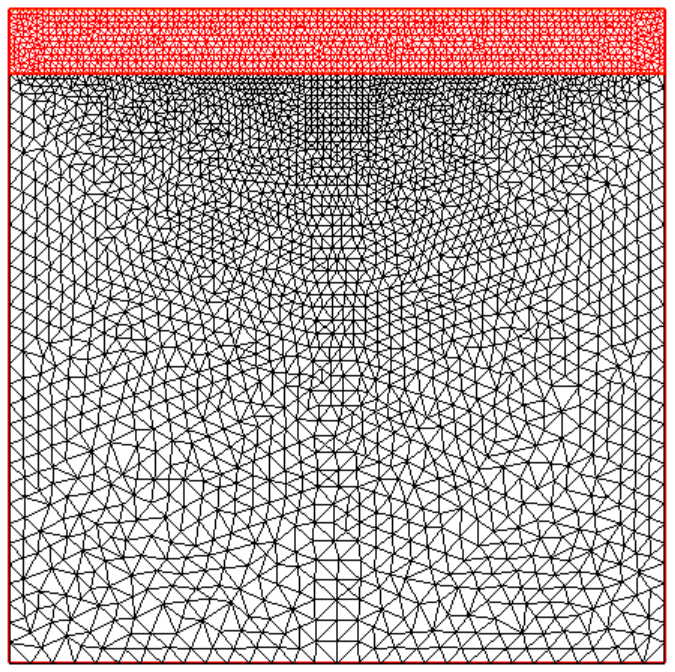
\includegraphics[width=0.5\textwidth]{imgs/confroming_mesh_100_30.PNG}
	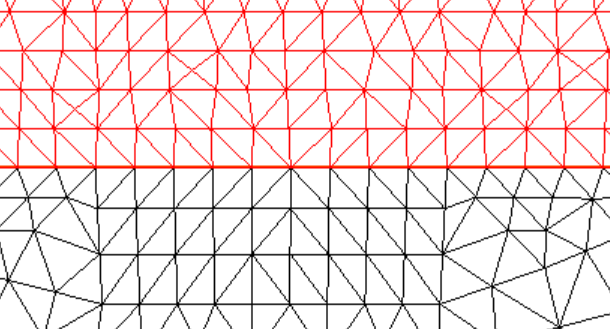
\includegraphics[width=0.5\textwidth]{imgs/conforming_mesh_intersection.PNG}
	\caption{Conforming mesh using
	N1=30 and N2=100}
\end{figure}
\begin{figure}[H] \label{fig:sol_conf}
	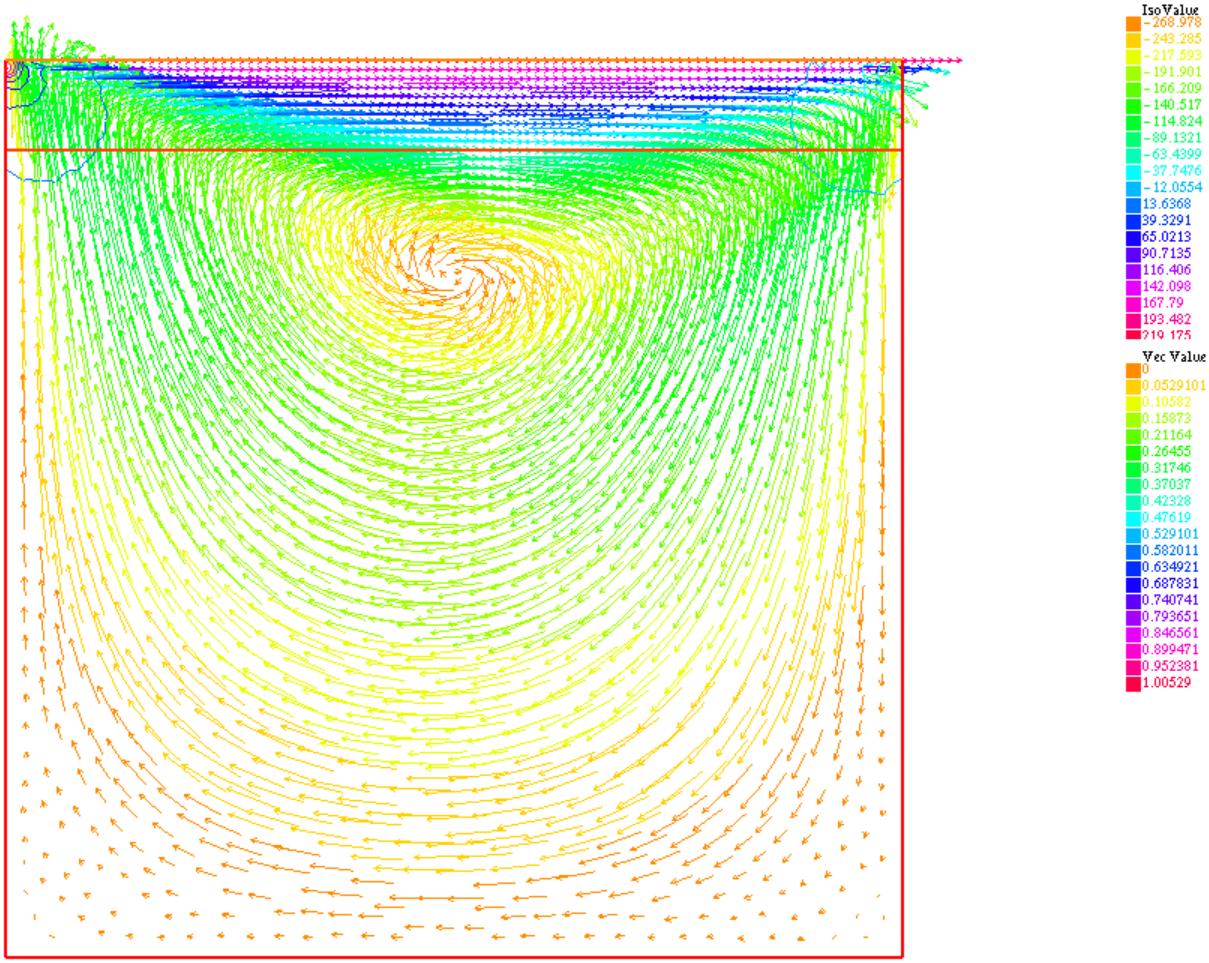
\includegraphics[width=0.5\textwidth]{imgs/solution-C_100_30.PNG}
	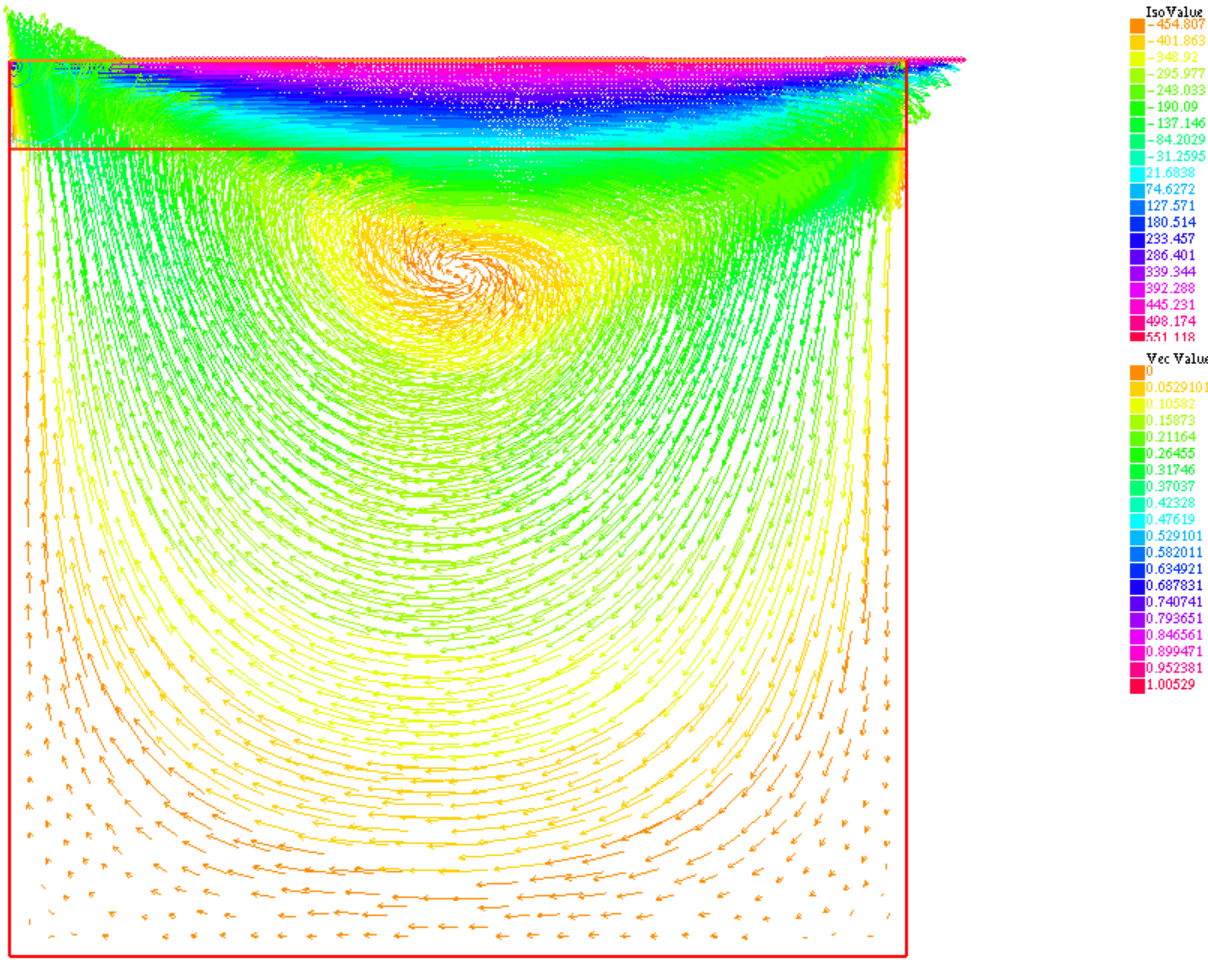
\includegraphics[width=0.5\textwidth]{imgs/solution-C_200_30.PNG}
	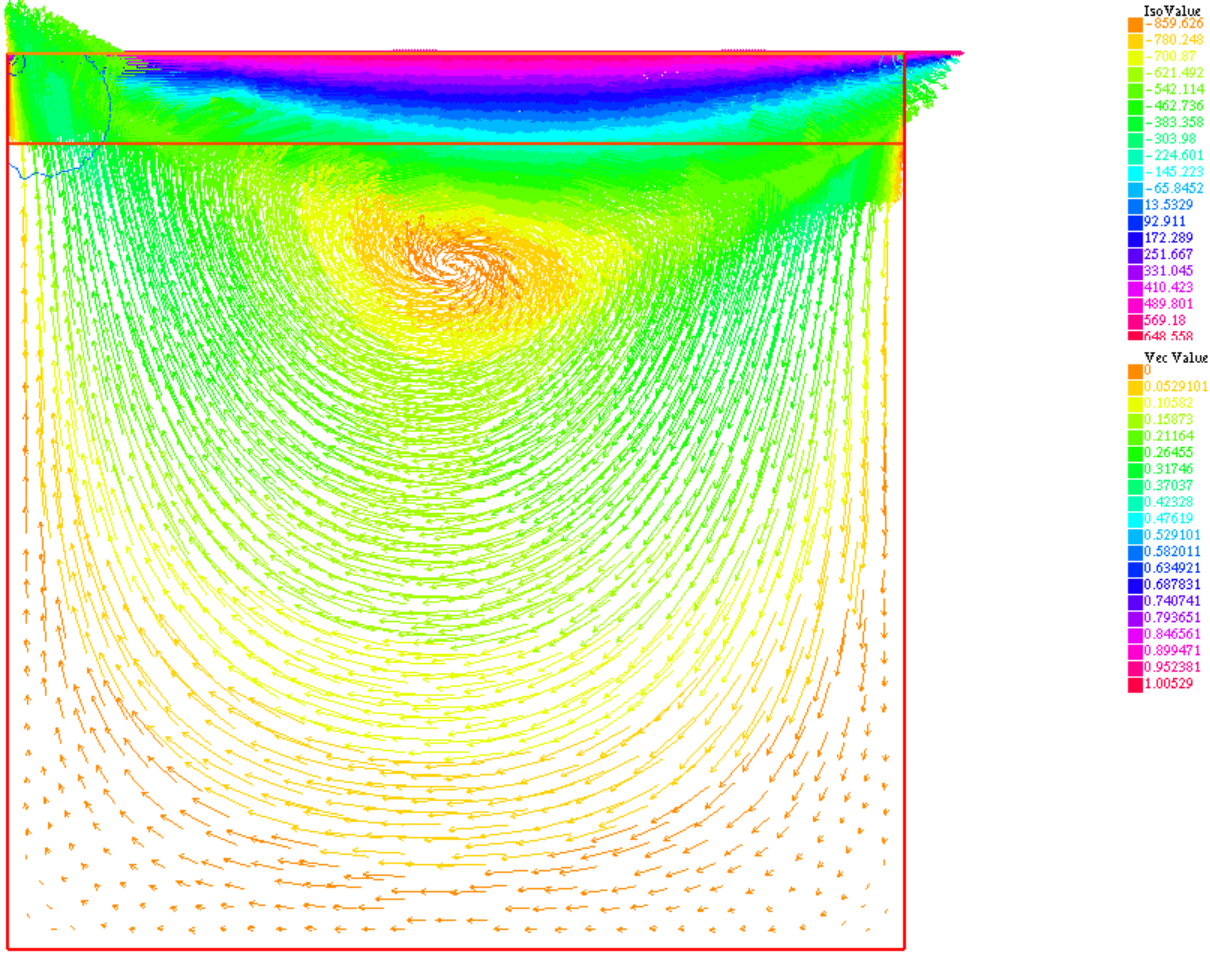
\includegraphics[width=0.5\textwidth]{imgs/solution-C_300_30.PNG}
	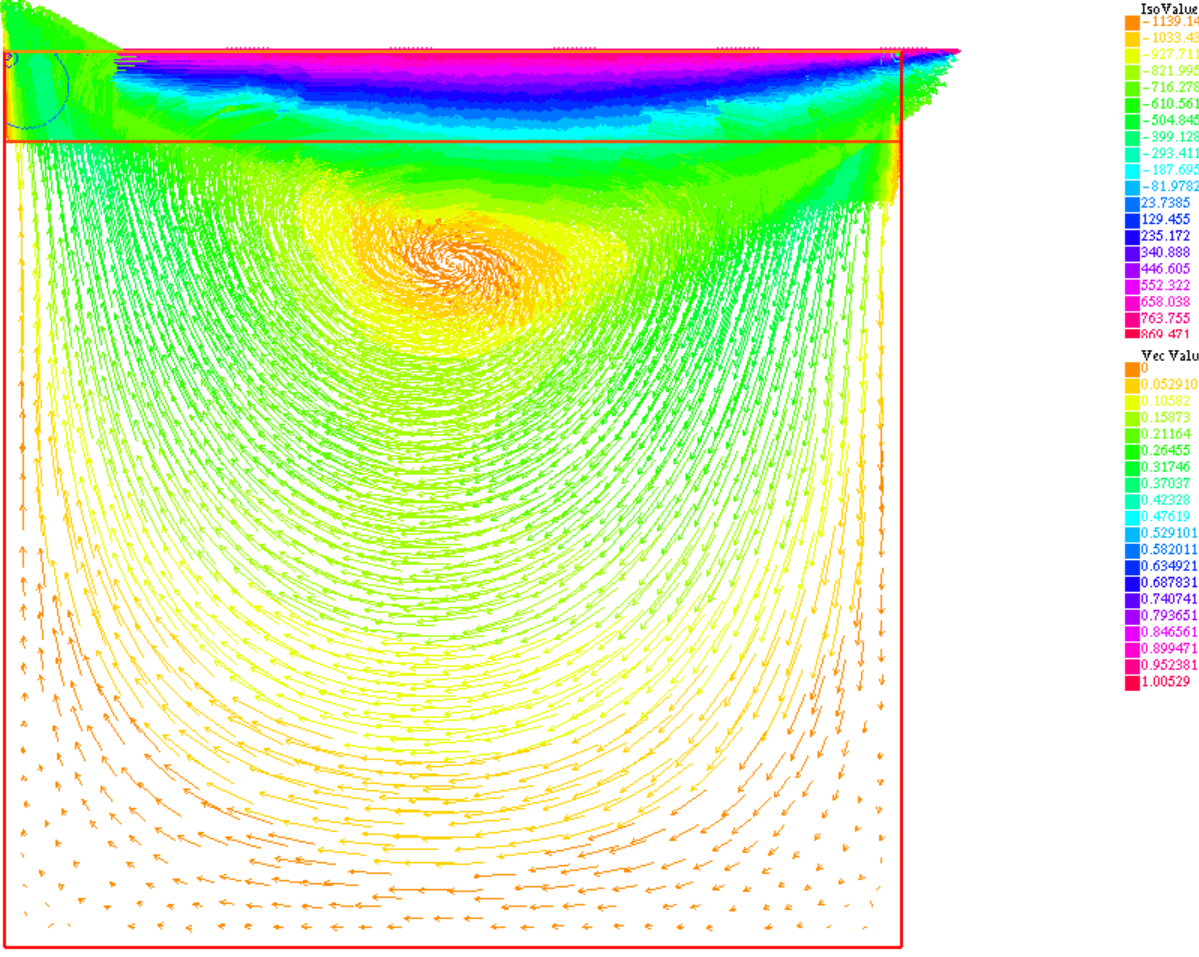
\includegraphics[width=0.5\textwidth]{imgs/solution-C_400_30.PNG}
	\caption{Solutions with conforming mesh for different mesh sizes: N1=30 and N2=100 (top left), N1=30 and N2=200 (top right), N1=30 and N2=300 (bottom left), N1=30 and N2=400 (bottom right)}
\end{figure}

\section*{Question 4}
To reach higher accuracy, we can also use two non-conforming meshes and connect
them thanks to Lagrange multipliers. Due to this separation, we can ask for
more precision where we need and release accuracy in the area without interest.
This is the so-called Mortar method with dual Lagrange multipliers. We
implemented this method and the code is as well given in the annex.

For the Lagrange multipliers, there has to be a certain mesh and corresponding
FEM space. The mesh just consists of the interface between the two domains, but
in FreeFEM++ this is not possible, so we took the mesh as the border of the
upper mesh. Then we used $\mathbb{P}_0$ elements for each multiplier which
ensure continuity on the normal and tangential components of the velocity. In
contrast to a conforming mesh, we now need two finite element spaces on two
different meshes defined independently. To deal with it we defined several
variational forms and extracted the associated matrix to reconstruct our
problem as a linear system.

To see the difference to the conforming mesh we tested it on similar mesh sizes, the results can be seen in figure \ref{fig:mesh_nonconf} and \ref{fig:sol_nonconf}.

Comparing these results to the previous ones, we can see that they are
similar, although the non-conforming case requires less computational effort. The
pressure is still diverging as expected when we refine the mesh. However, after a certain mesh size, the number of vectors is too high, and there is superposition, the result is too polluted to see meaningful differences, and we can no more rely on graphical observation. 

\begin{figure}[H] \label{fig:mesh_nonconf}
	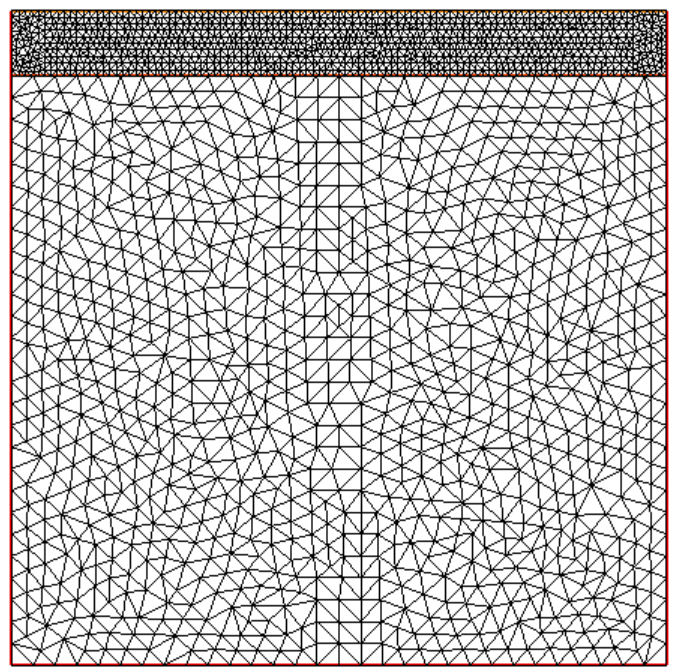
\includegraphics[width=0.5\textwidth]{imgs/non-confroming_mesh_100_30.PNG}
	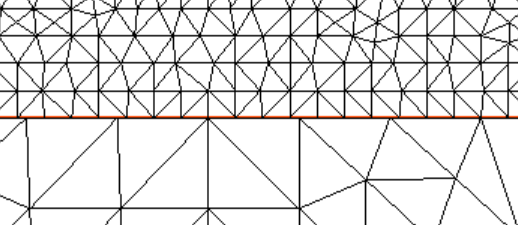
\includegraphics[width=0.5\textwidth]{imgs/non-conforming_mesh_intersection.PNG}
	\caption{Conforming mesh using
	N1=30 and N2=100}
\end{figure}
\begin{figure}[H] \label{fig:sol_nonconf}
	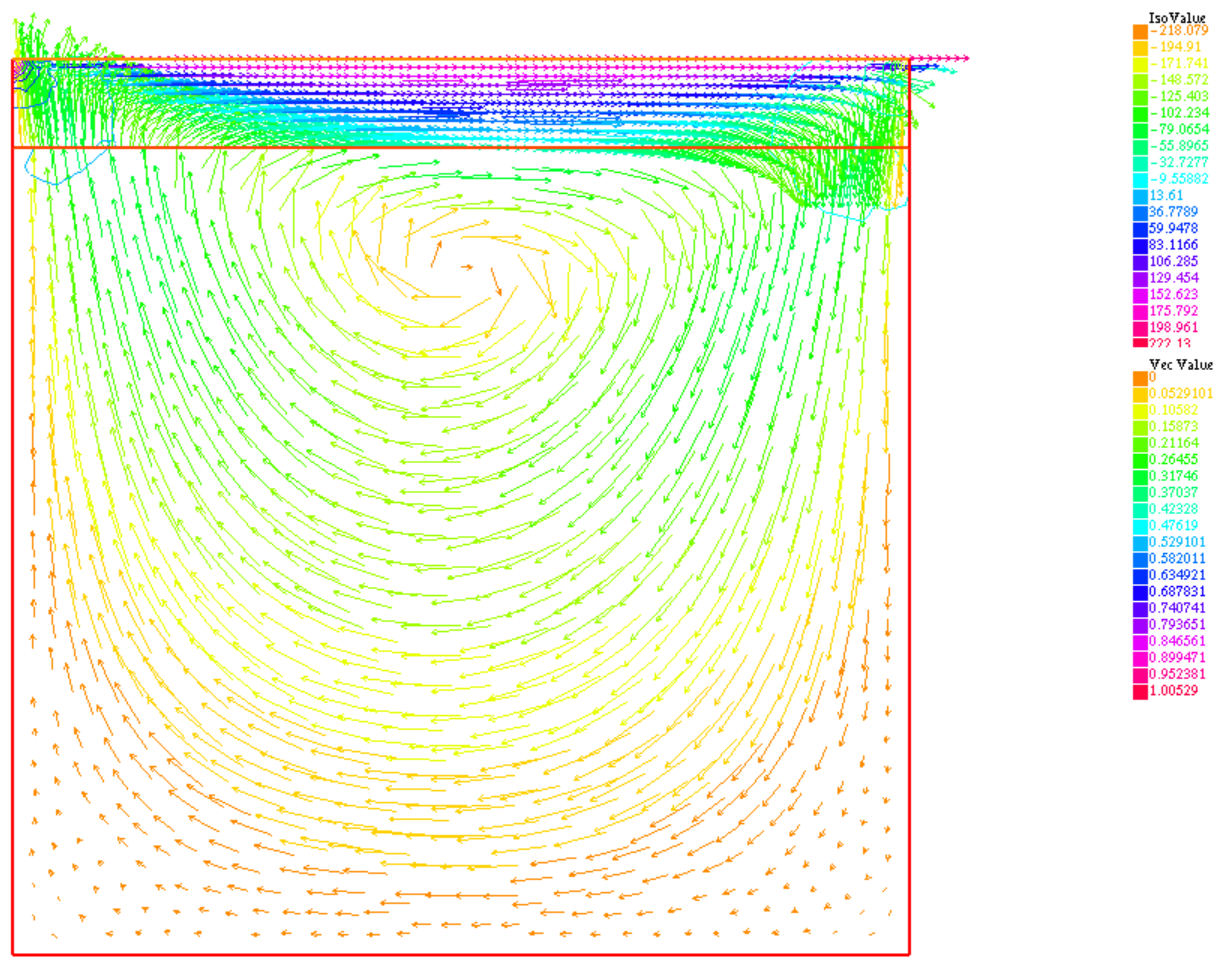
\includegraphics[width=0.5\textwidth]{imgs/solution-NC_100_30.PNG}
	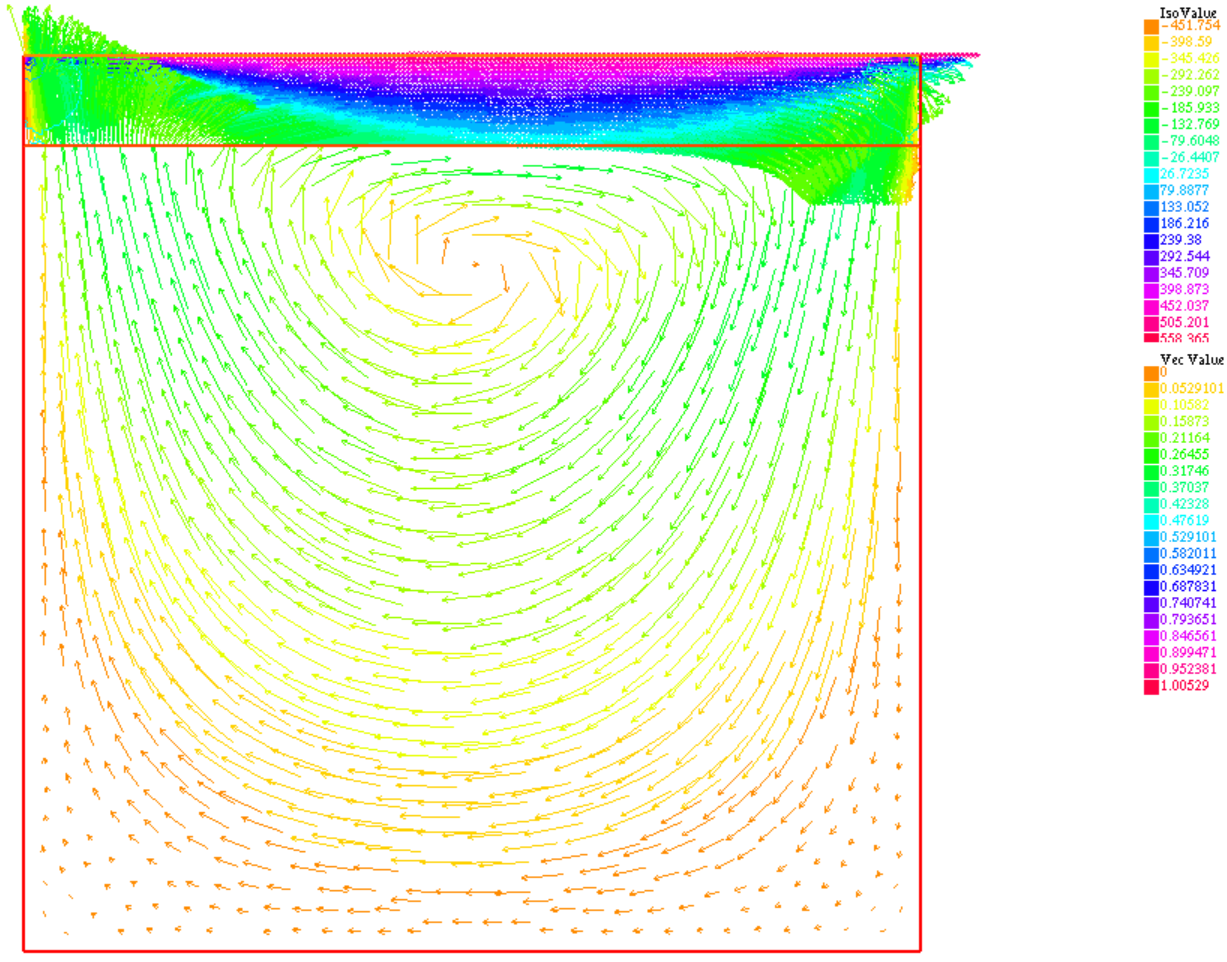
\includegraphics[width=0.5\textwidth]{imgs/solution-NC_200_30.PNG}
	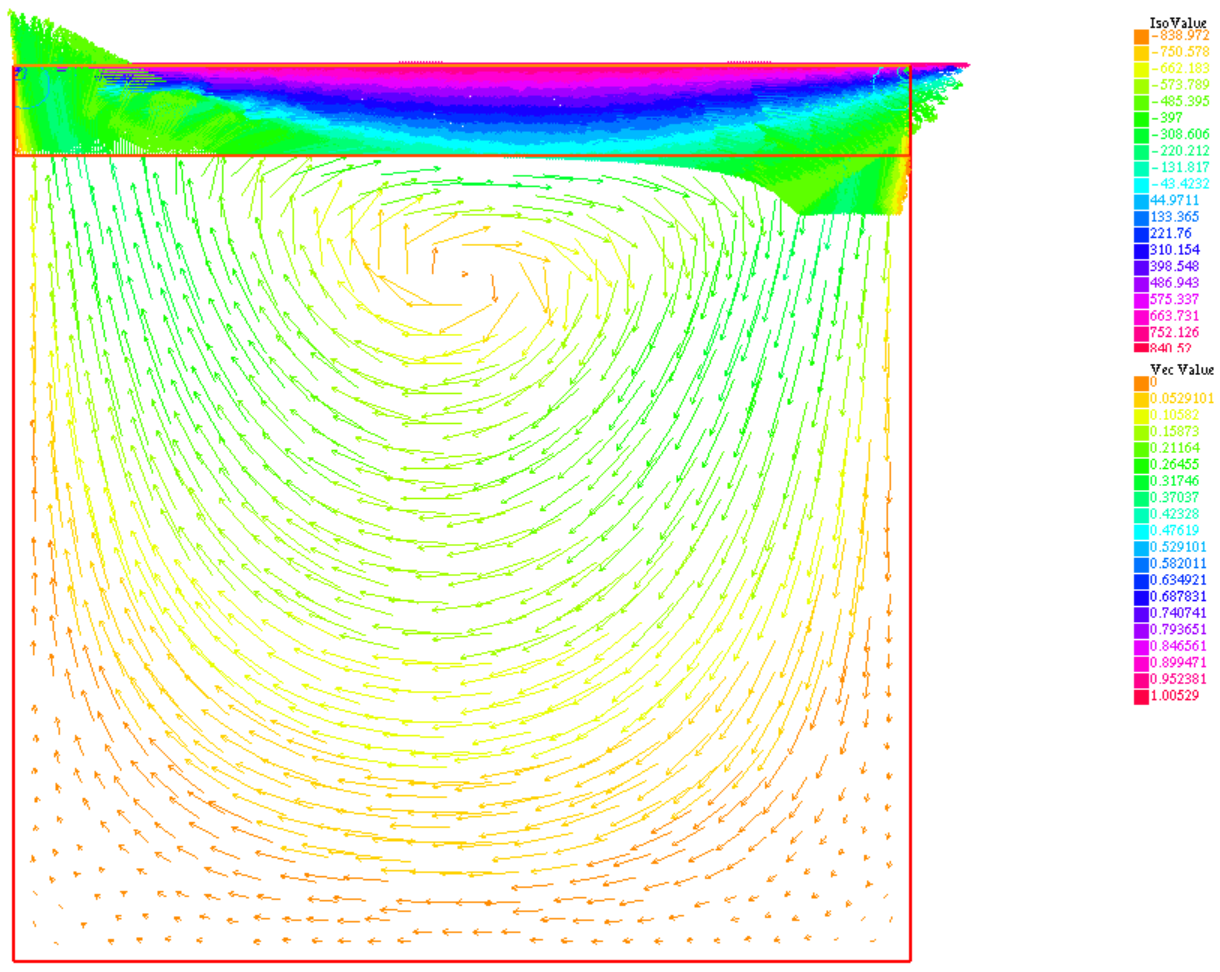
\includegraphics[width=0.5\textwidth]{imgs/solution-NC_300_30.PNG}
	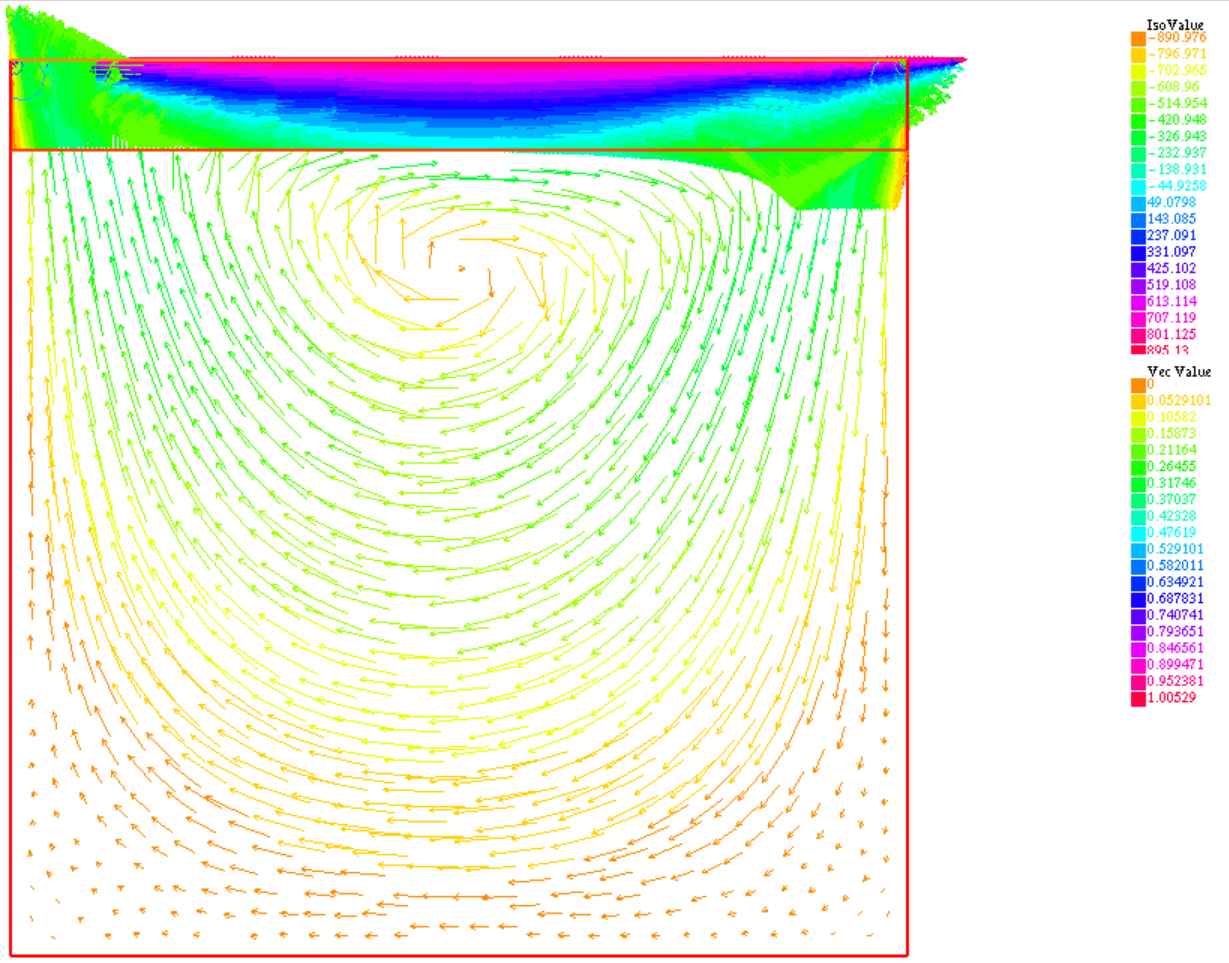
\includegraphics[width=0.5\textwidth]{imgs/solution-NC_400_30.PNG}
	\caption{Solutions with non conforming mesh for different mesh sizes: N1=30 and N2=100 (top left), N1=30 and N2=200 (top right), N1=30 and N2=300 (bottom left), N1=30 and N2=400 (bottom right)}
\end{figure}

\subsection*{Comparison between conforming and non-conforming meshs}
To compare the conforming and the non-conforming case we refined the upper rectangle (i.d setting N2) by fixing the lower part N1 to 30. It is important to note that the created graphs in figure \ref{comp_meshs} will not show an $h$ convergence as the comparing parameter is N2. The sole purpose of this computational experiment is to see if the mortar method (much less computational effort because of fewer nodes) will have an error similar to the one of the conforming mesh. As a reference solution, we used a mesh with 400 nodes per side without an interface.

\begin{figure}[H]
	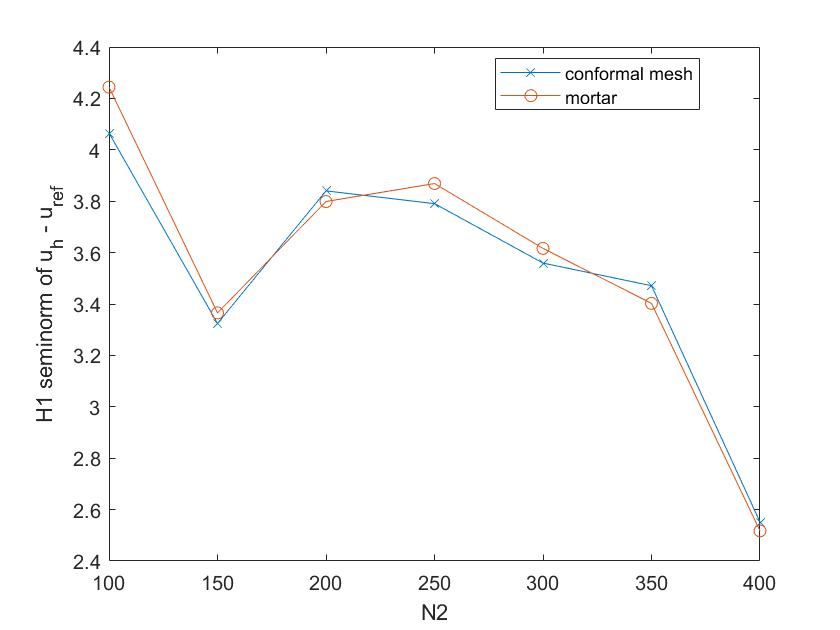
\includegraphics[width=0.5\textwidth]{imgs/errorH1.jpg}
	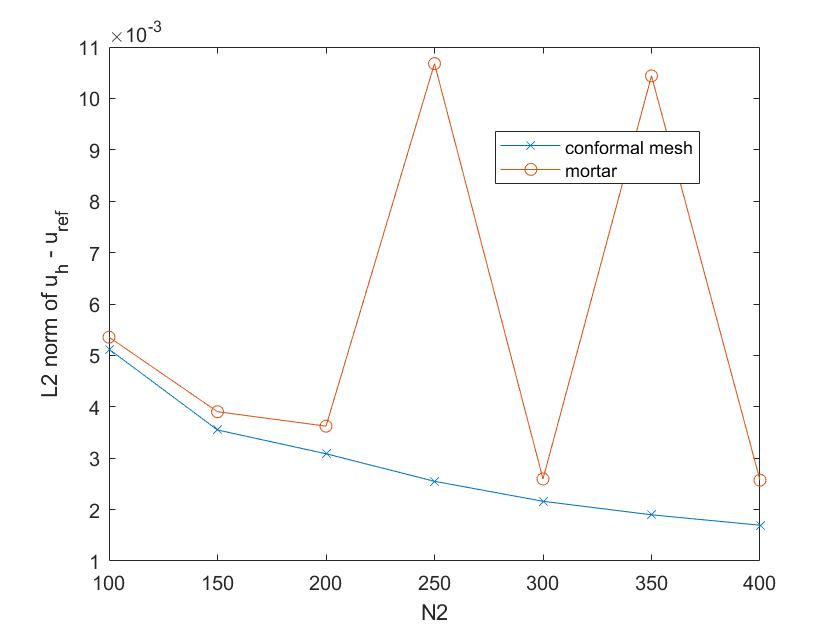
\includegraphics[width=0.5\textwidth]{imgs/errorL2.jpg}
	\caption{$H^1$ semi-norm and $L^2$ norm of velocity versus a reference solution, for conformal and non-conformal meshs}
	\label{comp_meshs}
\end{figure}

Thanks to these graphs we can see that the convergence between the two methods is similar. So to save the computational effort it seems reasonable to consider the mortar method. But the area of interest has to be well defined.

Interestingly the $L^2$ error for the Mortar method starts to oscillate which could be due to the coupling of the meshs and the numerical errors. Still the total error is small (~$10^{-3}$).

In general it is clear that the errors of the refinement won't converge to zero because firstly the reference solution is not analytically exact. Secondly the lower area is not refined while iterating. These causes for example the $H^1$ semi-norm to still stay at around $2.5$ after fully refining the top area to the same density of triangles as the reference solution.

\section*{Question 5}
We constructed a finite element space using the mini-element. This requires the pressure to be in $\mathbb{P}_1$. The pressure is forced to be continuous. If we allowed discontinuous pressure, some problems would arise. Indeed if we took the space $\mathbb{P}_0$ for pressure would be smaller and the problem would be affected by locking so the only solution would be $\mathbf{u}=0$ in $\Omega$ but it can not be a solution since we have boundary terms. On the contrary, if we took the space bigger, for example, $\mathbb{P}_1^{dc}$, the solution would be affected by spurious modes for pressure.

If we want discontinuous pressure, we have to find a new couple of finite element spaces, for which the inf-sup condition and coercivity on the kernel are still verified. A choice that is possible is the $\mathbb{P}_2$ / $\mathbb{P}_0$ element. The important point is that (both the just described space and the mini-element) are unbalanced for the quasi-optimal convergence in $p$ and $\mathbf{u}$. This results in a total convergence of $h$. Thus the mini-element is to prefer as we spend less computation for the velocity components.


\section*{Annex}
Below the code for solving the Stokes problem on a conforming and non-conforming are shown. The code used for the error analysis is included in the zip file.

\subsection*{Stokes on conforming mesh}
\begin{lstlisting} [language=C++]
	// parameters
	real eps = 1e-6; // for penalty method 

	real frac = 0.1; // fraction of side length in upper area
	int n2 = 100; // mesh size in upper area
	int n1 = 30; // mesh size in lower area

	// mesh
	border a1(t=0, 1){x=t; y=0; label=1;};
	border b1(t=0, 1-frac){x=1; y=t; label=1;};
	border c12(t=0, 1){x=1-t; y=1-frac; label=2;}; // border between areas
	border d1(t=frac, 1){x=0; y=1-t; label=1;};
	border a2(t=0, frac){x=1; y=1-frac+t; label=1;};
	border b2(t=0, 1){x=1-t; y=1; label=3;};
	border c2(t=0, frac){x=0; y=1-t; label=1;};

	mesh Th = buildmesh(a1(n1)+b1((1-frac)*n1)+c12(n2)+d1((1-frac)*n1)+a2(frac*n2)+b2(n2)+c2(frac*n2));

	plot(Th, wait=1);

	// fespaces
	fespace Xh(Th, [P1b, P1b, P1]);
	Xh [ux, uy, p], [vx, vy, q];
 	 
	// problem
	solve stokes ([ux, uy, p], [vx, vy, q])
		=   int2d(Th)(dx(ux)*dx(vx) + dy(ux)*dy(vx) + dx(uy)*dx(vy) + dy(uy)*dy(vy))
        - int2d(Th)(p*(dx(vx) + dy(vy)))

        - int2d(Th)(q*(dx(ux) + dy(uy)))
        - int2d(Th)(eps*p*q)

        + on(3, ux=1, uy=0)
      	+ on(1, ux=0, uy=0);

	// plot
	plot([ux, uy], p, value=true, wait=true);
\end{lstlisting}

\subsection*{Stokes on non-conforming mesh}
\begin{lstlisting} [language=C++]
	// parameters
	real eps = 1e-6; // for penalty method 

	real frac = 0.1; // fraction of side length of upper area
	int n2 = 100; // mesh size in upper area
	int n1 = 30; // mesh size in lower area

	// lower mesh
	border a1(t=0, 1){x=t; y=0; label=1;};
	border b1(t=0, 1-frac){x=1; y=t; label=1;};
	border c1(t=0, 1){x=1-t; y=1-frac; label=2;};
	border d1(t=frac, 1){x=0; y=1-t; label=1;};

	mesh Th1 = buildmesh(a1(n1)+b1((1-frac)*n1)+c1(n1)+d1((1-frac)*n1));

	// upper mesh
	border a2(t=0, frac){x=1;y=1-frac+t; label=1;};
	border b2(t=0, 1){x=1-t; y=1; label=3;};
	border c2(t=0, frac){x=0; y=1-t; label=1;};
	border d2(t=0, 1){x=t; y=1-frac; label=2;};

	mesh Th2 = buildmesh(a2(frac*n2)+b2(n2)+c2(frac*n2)+d2(n2));

	plot(Th1, Th2, wait=1);

	// interface mesh
	mesh interface = emptymesh(Th2);

	// lower fespaces and problem
	fespace Xh1(Th1, [P1b, P1b, P1]);
	Xh1[ux1, uy1, p1];

	varf stokes1([ux, uy, p], [vx, vy, q], solver=sparsesolver)
		=   int2d(Th1)(dx(ux)*dx(vx) + dy(ux)*dy(vx) + dx(uy)*dx(vy) + dy(uy)*dy(vy))
	  	  - int2d(Th1)(p*(dx(vx) + dy(vy)))

	  	  - int2d(Th1)(q*(dx(ux) + dy(uy)))
	  	  - int2d(Th1)(eps*p*q)

	  	  + on(1, ux=0, uy=0);

	// upper fespaces and problem
	fespace Xh2(Th2, [P1b, P1b, P1]);
	Xh2[ux2, uy2, p2];

	varf stokes2([ux, uy, p], [vx, vy, q], solver=sparsesolver)
		=   int2d(Th2)(dx(ux)*dx(vx) + dy(ux)*dy(vx) + dx(uy)*dx(vy) + dy(uy)*dy(vy))
	  	  - int2d(Th2)(p*(dx(vx) + dy(vy)))

	  	  - int2d(Th2)(q*(dx(ux) + dy(uy)))
	  	  - int2d(Th2)(eps*p*q)

	  	  + on(3, ux=1, uy=0)
	  	  + on(1, ux=0, uy=0);

	// interface fespace
	fespace Ih(interface, [P0, P0]);
	Ih [lambda, mu];

	// lagrange multipliers
	varf lagrange1([lambda, mu], [ux, uy, p], solver=sparsesolver) = int1d(Th2, 2)(uy*lambda-ux*mu);
	varf lagrange2([lambda, mu], [ux, uy, p], solver=sparsesolver) = int1d(Th2, 2)(-uy*lambda+ux*mu);

	// solving
	matrix A1 = stokes1(Xh1, Xh1);
	real[int] B1 = stokes1(0, Xh1);
	matrix A2 = stokes2(Xh2, Xh2);
	real[int] B2 = stokes2(0, Xh2);

	matrix L1 = lagrange1(Ih, Xh1);
	matrix L2 = lagrange2(Ih, Xh2);
	real[int] B3(Ih.ndof); B3 = 0;

	matrix A = [[A1, 0,L1],
		    	[0, A2, L2], 
		    	[L1',L2',0]];
	set(A, solver=sparsesolver);

	real[int] B = [B1, B2, B3];
	real[int] S1(Xh1.ndof), S2(Xh2.ndof), multipliers(Ih.ndof);
	real[int] sol = A^-1 * B;
	[S1, S2, multipliers] = sol;

	p1[] = S1;
	p2[] = S2;
	lambda[] = multipliers;

	// plot
	plot([ux1, uy1], p1,[ux2, uy2], p2,value=true, wait=true);
\end{lstlisting}

\bibliographystyle{IEEEtran}
\bibliography{bibliography.bib}

\end{document}
